\documentclass[12pt, a4paper, oneside]{ctexart}
\usepackage{amsmath, amsthm, amssymb, bm, color, graphicx, geometry, hyperref, mathrsfs,extarrows, braket, booktabs, array}

\linespread{1.5}
%\geometry{left=2.54cm,right=2.54cm,top=3.18cm,bottom=3.18cm}
\geometry{left=1.84cm,right=1.84cm,top=2.18cm,bottom=2.18cm}
\newenvironment{problem}{\par\noindent\textbf{题目. }}{\bigskip\par}
\newenvironment{solution}{\par\noindent\textbf{解答. }}{\bigskip\par}
\newenvironment{note}{\par\noindent\textbf{注记. }}{\bigskip\par}

% 基本信息
\newcommand{\RQ}{\today} % 日期
\newcommand{\km}{数值分析} % 科目
\newcommand{\bj}{强基数学002} % 班级
\newcommand{\xm}{吴天阳} % 姓名
\newcommand{\xh}{2204210460} % 学号
\newcommand{\XH}{59} % 序号

\begin{document}

%\pagestyle{empty}
\pagestyle{plain}
\vspace*{-15ex}
\centerline{\begin{tabular}{*6{c}}
    \parbox[t]{0.25\linewidth}{\begin{center}\textbf{日期}\\ \large \textcolor{blue}{\RQ}\end{center}} 
    & \parbox[t]{0.15\linewidth}{\begin{center}\textbf{科目}\\ \large \textcolor{blue}{\km}\end{center}}
    & \parbox[t]{0.2\linewidth}{\begin{center}\textbf{班级}\\ \large \textcolor{blue}{\bj}\end{center}}
    & \parbox[t]{0.1\linewidth}{\begin{center}\textbf{姓名}\\ \large \textcolor{blue}{\xm}\end{center}}
    & \parbox[t]{0.15\linewidth}{\begin{center}\textbf{学号}\\ \large \textcolor{blue}{\xh}\end{center}}
    & \parbox[t]{0.1\linewidth}{\begin{center}\textbf{序号}\\ \large \textcolor{blue}{\XH}\end{center}} \\ \hline
\end{tabular}}
\vspace*{4ex}
\def\disp{\displaystyle}
\paragraph{第六章}
\paragraph{6.2}取$n=8$,用复化梯形、复化辛普森求积公式计算积分$\disp\int_0^1\frac{1}{1+x}\,dx$,保留$7$位小数。
\begin{solution}
    \begin{equation*}
        \begin{aligned}
            T_8 =&\ \frac{1}{16}\left(1+2\left(\frac{1}{1+\frac{1}{8}}+\frac{1}{1+\frac{2}{8}}+\cdots+\frac{1}{1+\frac{7}{8}}\right)+\frac{1}{1+2}\right)\\
            =&\ \frac{1}{12}+\left(\frac{1}{9}+\frac{1}{10}+\cdots+\frac{1}{15}\right)\approx 0.6837052\\
            S_8 =&\ \frac{1}{48}\left(16T_8+4\left(\frac{1}{1+\frac{1}{16}}+\frac{1}{1+\frac{3}{16}}+\cdots+\frac{1}{1+\frac{15}{16}}\right)\right)\\
            =&\ \frac{T_8}{3}+\frac{4}{3}\left(\frac{1}{17}+\frac{1}{19}+\cdots+\frac{1}{31}\right))\approx 0.6896754
        \end{aligned}
    \end{equation*}
\end{solution}
\paragraph{6.4}若用复化梯形求积公式计算积分$\disp I = \int_0^1e^x\,dx$,问区间$[0,1]$分成多少等份,才能使截断误差不超过$\disp\frac{1}{2}\times 10^{-5}$?若改用复化辛普森求积公式计算,要达到同样的精度,区间$[0,1]$应分成多少等份?
\begin{solution}
    由于$\disp\max_{x\in[0,1]}(e^{x})^(k) = e\ (\forall k\in \mathbb{N})$,设$\disp h = \frac{1}{n}$,则
    \begin{equation*}
        \begin{aligned}
            |R_{T_n}[f]| =&\ \frac{1}{12}h^2|f''(\eta)|\leqslant \frac{1}{12}h^2e\leqslant \frac{1}{2}\times10^{-5}\Rightarrow n\geqslant \left[\left(\frac{e\times 10^5}{6}\right)^{1/2}\right]+1\Rightarrow n\geqslant 213\\
            |R_{S_n}[f]| =&\ \frac{1}{2880}h^4|f''(\eta)|\leqslant \frac{1}{2880}h^4e\leqslant \frac{1}{2}\times10^{-5}\Rightarrow n\geqslant \left[\left(\frac{e\times 10^5}{1440}\right)^{1/4}\right]+1\Rightarrow n\geqslant 4
        \end{aligned}
    \end{equation*}
    所以,要使截断误差不超过$\disp\frac{1}{2}\times10^{-5}$,复化梯形求积公式至少需要$213$等分,而复化辛普森求积公式只需要$4$等分。
\end{solution}
\paragraph{6.7}导出下列求积公式及其截断误差估计式:

(1) $\disp\int_0^hf(x)\,dx\approx A_0f(0)+B_0f'(0)+A_1f(h)+B_1f'(h)$;

(2) $\disp\int_0^{2h}f(x)\,dx\approx A_0f(0)+A_1f(h)+A_2f(2h)$;

(3) $\disp\int_{-1}^1x^2f(x)\,dx\approx A_0f(x_0)+A_1f(x_1)$.

\begin{solution}
    (1) 取$f(x) = 1, x, x^2, x^3$,可得
    \begin{equation*}
        \begin{cases}
            h=A_0+A_1\\
            \frac{1}{2}h^2=B_0+A_1h+B_1\\
            \frac{1}{3}h^3=A_1h^2+2B_1h\\
            \frac{1}{4}h^4=A_1h^3+3B_1h^2
        \end{cases}
        \Rightarrow\quad\begin{cases}
            A_0 = A_1 = \frac{1}{2}h\\
            B_0 = \frac{1}{12}h^2\\
            B_1=-\frac{1}{12}h^2
        \end{cases}
    \end{equation*}
    则$\disp \int_0^hf(x)\,dx\approx\frac{h}{12}[6f(0)+hf'(0)+6f(h)-hf'(h)]$,由于
    \begin{equation*}
        I[x^4]=\int_0^hx^4\,dx = \frac{1}{5}h^5,\quad Q[x^4]=\frac{h}{12}[6h^4-4h^4] = \frac{h^5}{6},\quad R[x^4] = I[x^4] - Q[x^4] = \frac{1}{30}h^5\neq 0
    \end{equation*}
    所以该求积公式的代数精度$m=3$,令$\disp e(x) = \frac{f^{(4)}(\xi)}{4!}x^2(x-h)^2$,由广义Peano定理可知,截断误差为
    \begin{equation*}
        R[f] = R[e] = I[e] - Q[e] = \int_0^h\frac{f^{(4)}(\xi)}{4!}x^2(x-h)^2\,dx = \frac{f^{(4)}(\eta)}{720}h^5,\quad(\eta\in[0,h])
    \end{equation*}

    (2) 取$\disp f(x) = 1,x, x^2$,可得
    \begin{equation*}
        \begin{cases}
            2h = A_0+A_1+A_2\\
            2h^2=A_1h+2A_2h\\
            \frac{8}{3}h^3 = A_1h^2+4A_2h^2
        \end{cases}
        \Rightarrow\quad\begin{cases}
            A_0 = A_2 = \frac{1}{3}h\\
            A_1 = \frac{4}{3}h
        \end{cases}
    \end{equation*}
    则$\disp \int_0^{2h}f(x)\,dx = \frac{1}{3}hf(0)+\frac{4}{3}hf(h)+\frac{1}{3}hf(2h) = \frac{h}{3}[f(0)+4f(h)+f(2h)]$,由于
    \begin{equation*}
        \begin{aligned}
            I[x^3] =&\ \frac{(2h)^4}{4} = 4h^4,\quad Q[x^3] = \frac{h}{3}[4h^3+8h^3]=4h^4,\quad R[x^3] = I[x^3]-Q[x^3] = 0\\
            I[x^4] =&\ \frac{(2h)^5}{5} = \frac{32h^5}{5},\quad Q[x^4]=\frac{h}{3}[4h^4+16h^4]=\frac{20}{3}h^4,\quad R[x^4] = I[x^4]-Q[x^4] = -\frac{4}{15}h^4 \neq 0
        \end{aligned}
    \end{equation*}
    所以该求积公式的代数精度$m = 3$,令$\disp e(x) = \frac{f^{(4)}(\xi)}{4!}x(x-h)^2(x-2h)$,由广义Peano定理可知,截断误差为
    \begin{equation*}
        R[f] = R[e] = I[e] - Q[e] = \int_0^{2h}\frac{f^{(4)}(\xi)}{4!}x(x-h)^2(x-2h) = -\frac{f^{(4)}(\eta)}{90}h^5,\quad(\eta\in[0,2h])
    \end{equation*}

    (3) 这是$n=1$的高斯型求积公式,其代数精度$m  =2n+1 = 3$,所以求积公式对$f(x) = 1,x,x^2,x^3$准确成立,则
    \begin{equation*}
        \begin{cases}
            \frac{2}{3} = A_0+A_1\\
            0=A_0x_0+A_1x_1\\
            \frac{2}{5} = A_0x_0^2+A_1x_1^2\\
            0 = A_0x_0^3+A_1x_1^3
        \end{cases}\Rightarrow\quad \begin{cases}
            x_0 = -\frac{\sqrt{15}}{5}\\
            x_1 = \frac{\sqrt{15}}{5}\\
            A_0 = A_1 = \frac{1}{3}
        \end{cases}
    \end{equation*}
    则$\disp \int_{-1}^1x^2f(x)\,dx \approx \frac{1}{3}\left(f(-\frac{\sqrt{15}}{5})+f(\frac{\sqrt{15}}{5})\right)$,代数精度$m=3$,取
    \begin{equation*}
    e(x) = \frac{f^{(4)}(\xi)}{4!}(x+\frac{\sqrt{15}}{5})^2(x-\frac{\sqrt{15}}{5})^2 = \frac{f^{(4)}(\xi)}{4!}(x^2-\frac{3}{5})^2
    \end{equation*}
    由广义Peano定理可知, 截断误差为
    \begin{equation*}
        R[f] = R[e] = I[e] - Q[e] = \int_{-1}^1\frac{f^{(4)}{(\xi)}}{4!}(x^2-\frac{3}{5})^2=\frac{4}{75}f^{(4)}(\eta),\quad(\eta\in[-1,1])
    \end{equation*}
\end{solution}
\paragraph{6.10}确定下列数值微分公式的系数, 并导出截断误差表示式:

(1) $\disp f'(0)\approx af(-h)+bf(0)+cf(h);$

(2) $f'(h)\approx af'(0) + b[f(2h)-f(h)].$
\begin{solution}
    (1) 取$f(x) = 1, x, x^2$, 则
    \begin{equation*}
        \begin{cases}
            0 = a+b+c\\
            1=-ah+ch\\
            0=ah^2+ch^2
        \end{cases}\Rightarrow\quad\begin{cases}
            a = \frac{3}{2h}\\
            b = -\frac{2}{h}\\
            c = \frac{1}{2h}
        \end{cases}
    \end{equation*}
    则$\disp f'(0)\approx \frac{1}{2h}(3f(-h)-4f(0)+f(h))$, 由于$\disp R[x^3] = 0 - \frac{1}{2h}\left(3(-h)^3+h^3\right) = h^2 \neq 0$, 所以代数精度$m=2$, 令$\disp e(x) = \frac{f^{(3)}(\xi)}{3!}x(x+h)(x-h)$, 由广义Peano定理可知
    \begin{equation*}
        R[f] = R[e] = e'(0) = -\frac{h^2}{3!}f^{(3)}(\xi)
    \end{equation*}

    (2) 取$f(x) = 1, x, x^2$, 则
    \begin{equation*}
        \begin{cases}
            0 = 0\\
            1 = a + hb\\
            2h = 3h^2 b
        \end{cases}\Rightarrow\quad\begin{cases}
            a = \frac{1}{3}\\
            b = \frac{2}{3h}
        \end{cases}
    \end{equation*}
    则$\disp f'(h)\approx\frac{1}{3h}[hf'(0)+2f(2h)-2f(h)]$, 由于$\disp R[x^3] = 3h^2-\frac{1}{3h}(14h^3) = -\frac{5}{3}h^2\neq 0$, 所以代数精度$m=2$, 令$\disp e(x) = \frac{f^{(3)}(\xi)}{3!}x(x-2h)(x-h)$, 由广义Peano定理可知
    \begin{equation*}
        R[f] = R[e] = e'(h) - \frac{f^{(3)}(\xi)}{3!}\,\frac{2h^2}{3} = -\frac{5h^2}{18}f^{(3)}(\xi)
    \end{equation*}
\end{solution}

\iffalse
% 图片模板
\centerline{
    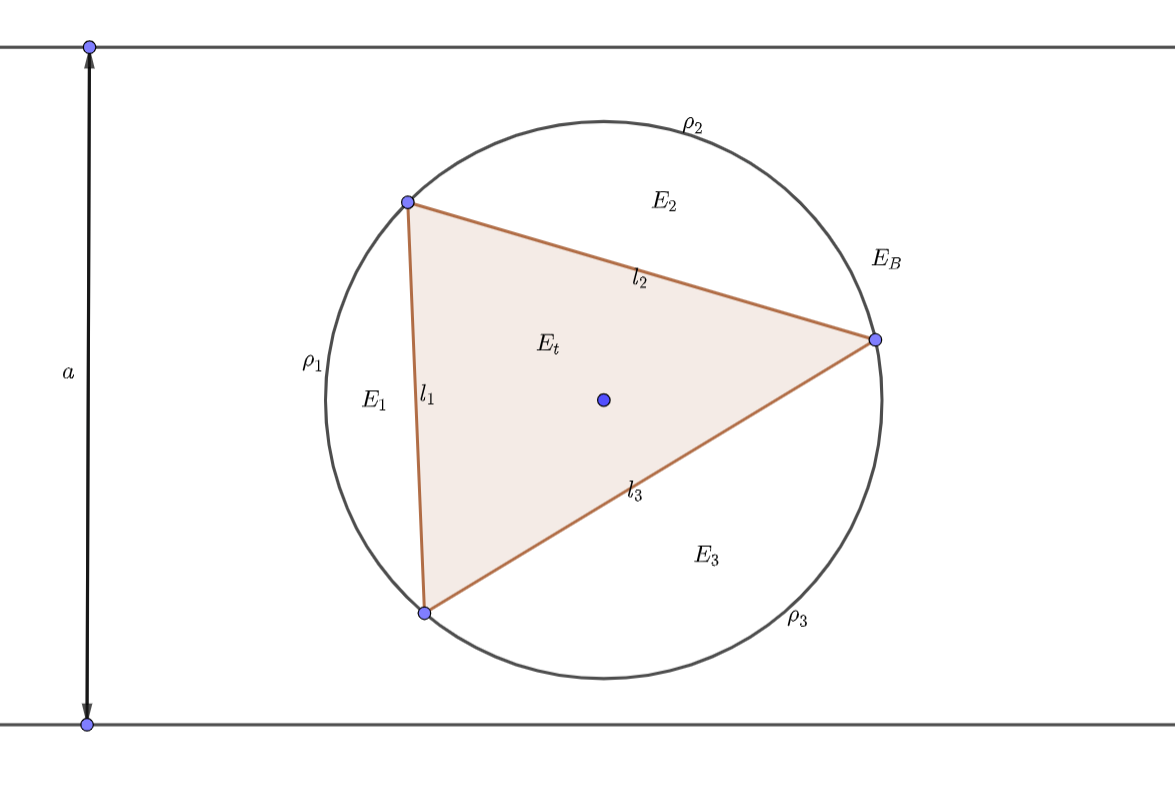
\includegraphics[width=0.8\textwidth]{figure.png}
}
\fi
\iffalse
% 表格模板
\renewcommand\arraystretch{0.8} % 设置表格高度为原来的0.8倍
\begin{table}[!htbp] % table标准
    \centering % 表格居中
    \begin{tabular}{p{1cm}<{\centering}p{1cm}<{\centering}p{3cm}<{\centering}p{5cm}<{\centering}} % 设置表格宽度
    %\begin{tabular}{cccc}
        \toprule
        $x_i$ & $f[x_1]$ & $f[x_i,x_{i+1}]$ & $f[x_i,x_{i+1},x_{i+2}]$ \\
        \midrule
        $x_0$ & $f(x_0)$ &                  &                          \\
        $x_0$ & $f(x_0)$ & $f'(x_0)$        &                          \\
        $x_0$ & $f(x_1)$ & $\frac{f(x_1)-f(x_0)}{x_1-x_0}$ & $\frac{f(x_1)-f(x_0)}{(x_1-x_0)^2}-\frac{f'(x_0)}{x_1-x_0}$\\
        \bottomrule
    \end{tabular}
\end{table}

\def\Log{\text{Log}} % 一个简单的宏定义
$\Log$ % 调用方法
\fi

\end{document}